\section{Onion}
\begin{frame}{Onion}
    \begin{figure}[htpb!]
        \centering
        \includesvg[width=\textwidth]{SpiegazioneOnion}
    \end{figure}
    La rete Onion è una rete distribuita composta da nodi chiamati \textbf{Onion Router}, collegati tra loro tramite i circuiti creati dagli \textbf{Onion Proxy}. \\
    Ogni pacchetto che passa nel circuito viene decriptato in maniera sequenziale dai relativi nodi fino ad arrivare all'exit node che si occupa di instradare il pacchetto nella rete Internet. \\ 
    Grazie a questo meccanismo nessun nodo conosce contemporaneamente l'indirizzo del mittente e del destinatario.
\end{frame}

\subsection{Creazione del circuito}
\begin{frame}{Creazione del circuito}
    La generazione del circuito è un processo \textbf{iterativo} e \textbf{progressivo} in cui il proxy sceglie i nodi del circuito. 
    A partire dal primo nodo viene instaurata una connessione \textbf{TLS} e vengono scambiate le \textbf{chiavi simmetriche} tramite un processo \textbf{asimmetrico} (in maniera simile allo scambio di chiavi di HTTPS). \\
    Questo processo continua fino all'exit node, a questo punto il circuito è completo e può iniziare a trasmettere stream dati.
\end{frame}
    
\begin{frame}
    \begin{figure}[htpb!]
        \centering
        \includesvg[width=\textwidth]{circuitCreation.svg}
    \end{figure}
\end{frame}

% Wireshark ci permette di vedere come viene generata la connessione \textbf{TLS}, in cui il client invia alcune informazioni tra cui la versione TLS, la lista dei Cipher Suite supportati e la chiave pubblica.
% Il proxy riceve poi il Server Hello, ovvero la risposta del server con le relative informazioni di criptografia. \\
% Successivamente Tor usa le informazioni ottenute per stabilire una connessione TLS tra client e server, impedendoci di vedere il traffico dati.
\begin{frame}{Dimostrazione Wireshark}
    \begin{figure}[htbp]
        \begin{subfigure}[c]{0.5\textwidth}
            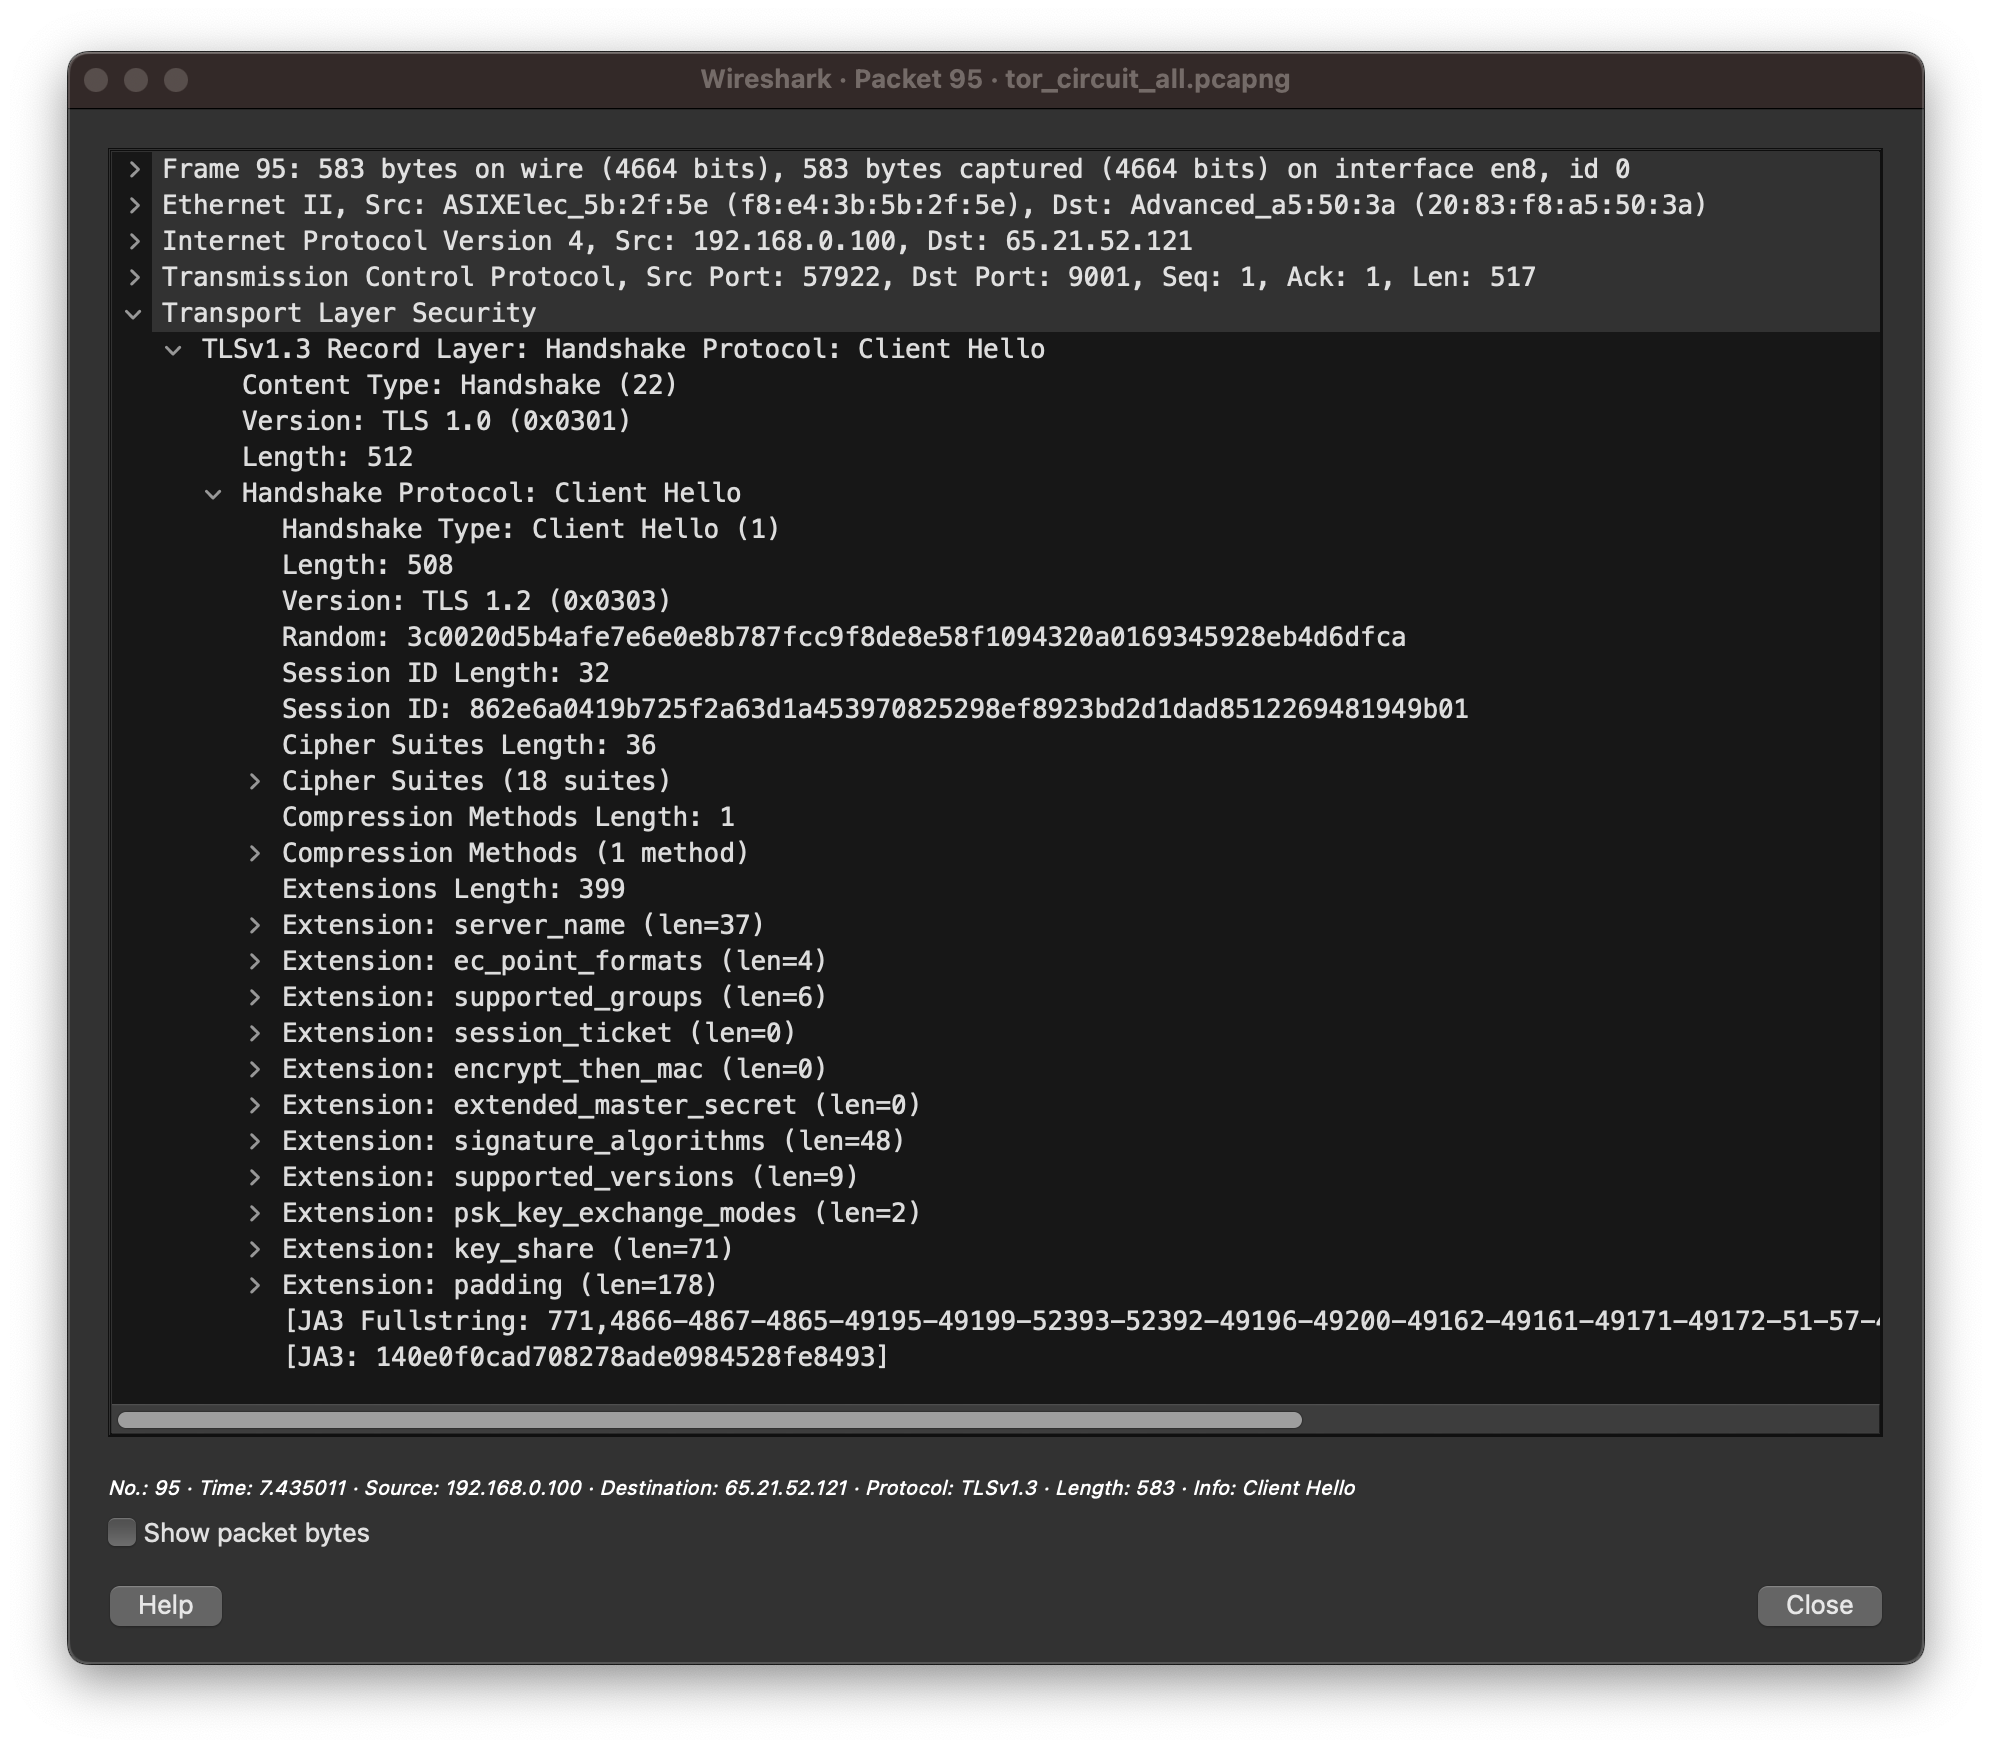
\includegraphics[width=\textwidth]{Wireshark/Client_Hello}
        \end{subfigure}
        \begin{subfigure}[c]{0.49\textwidth}
            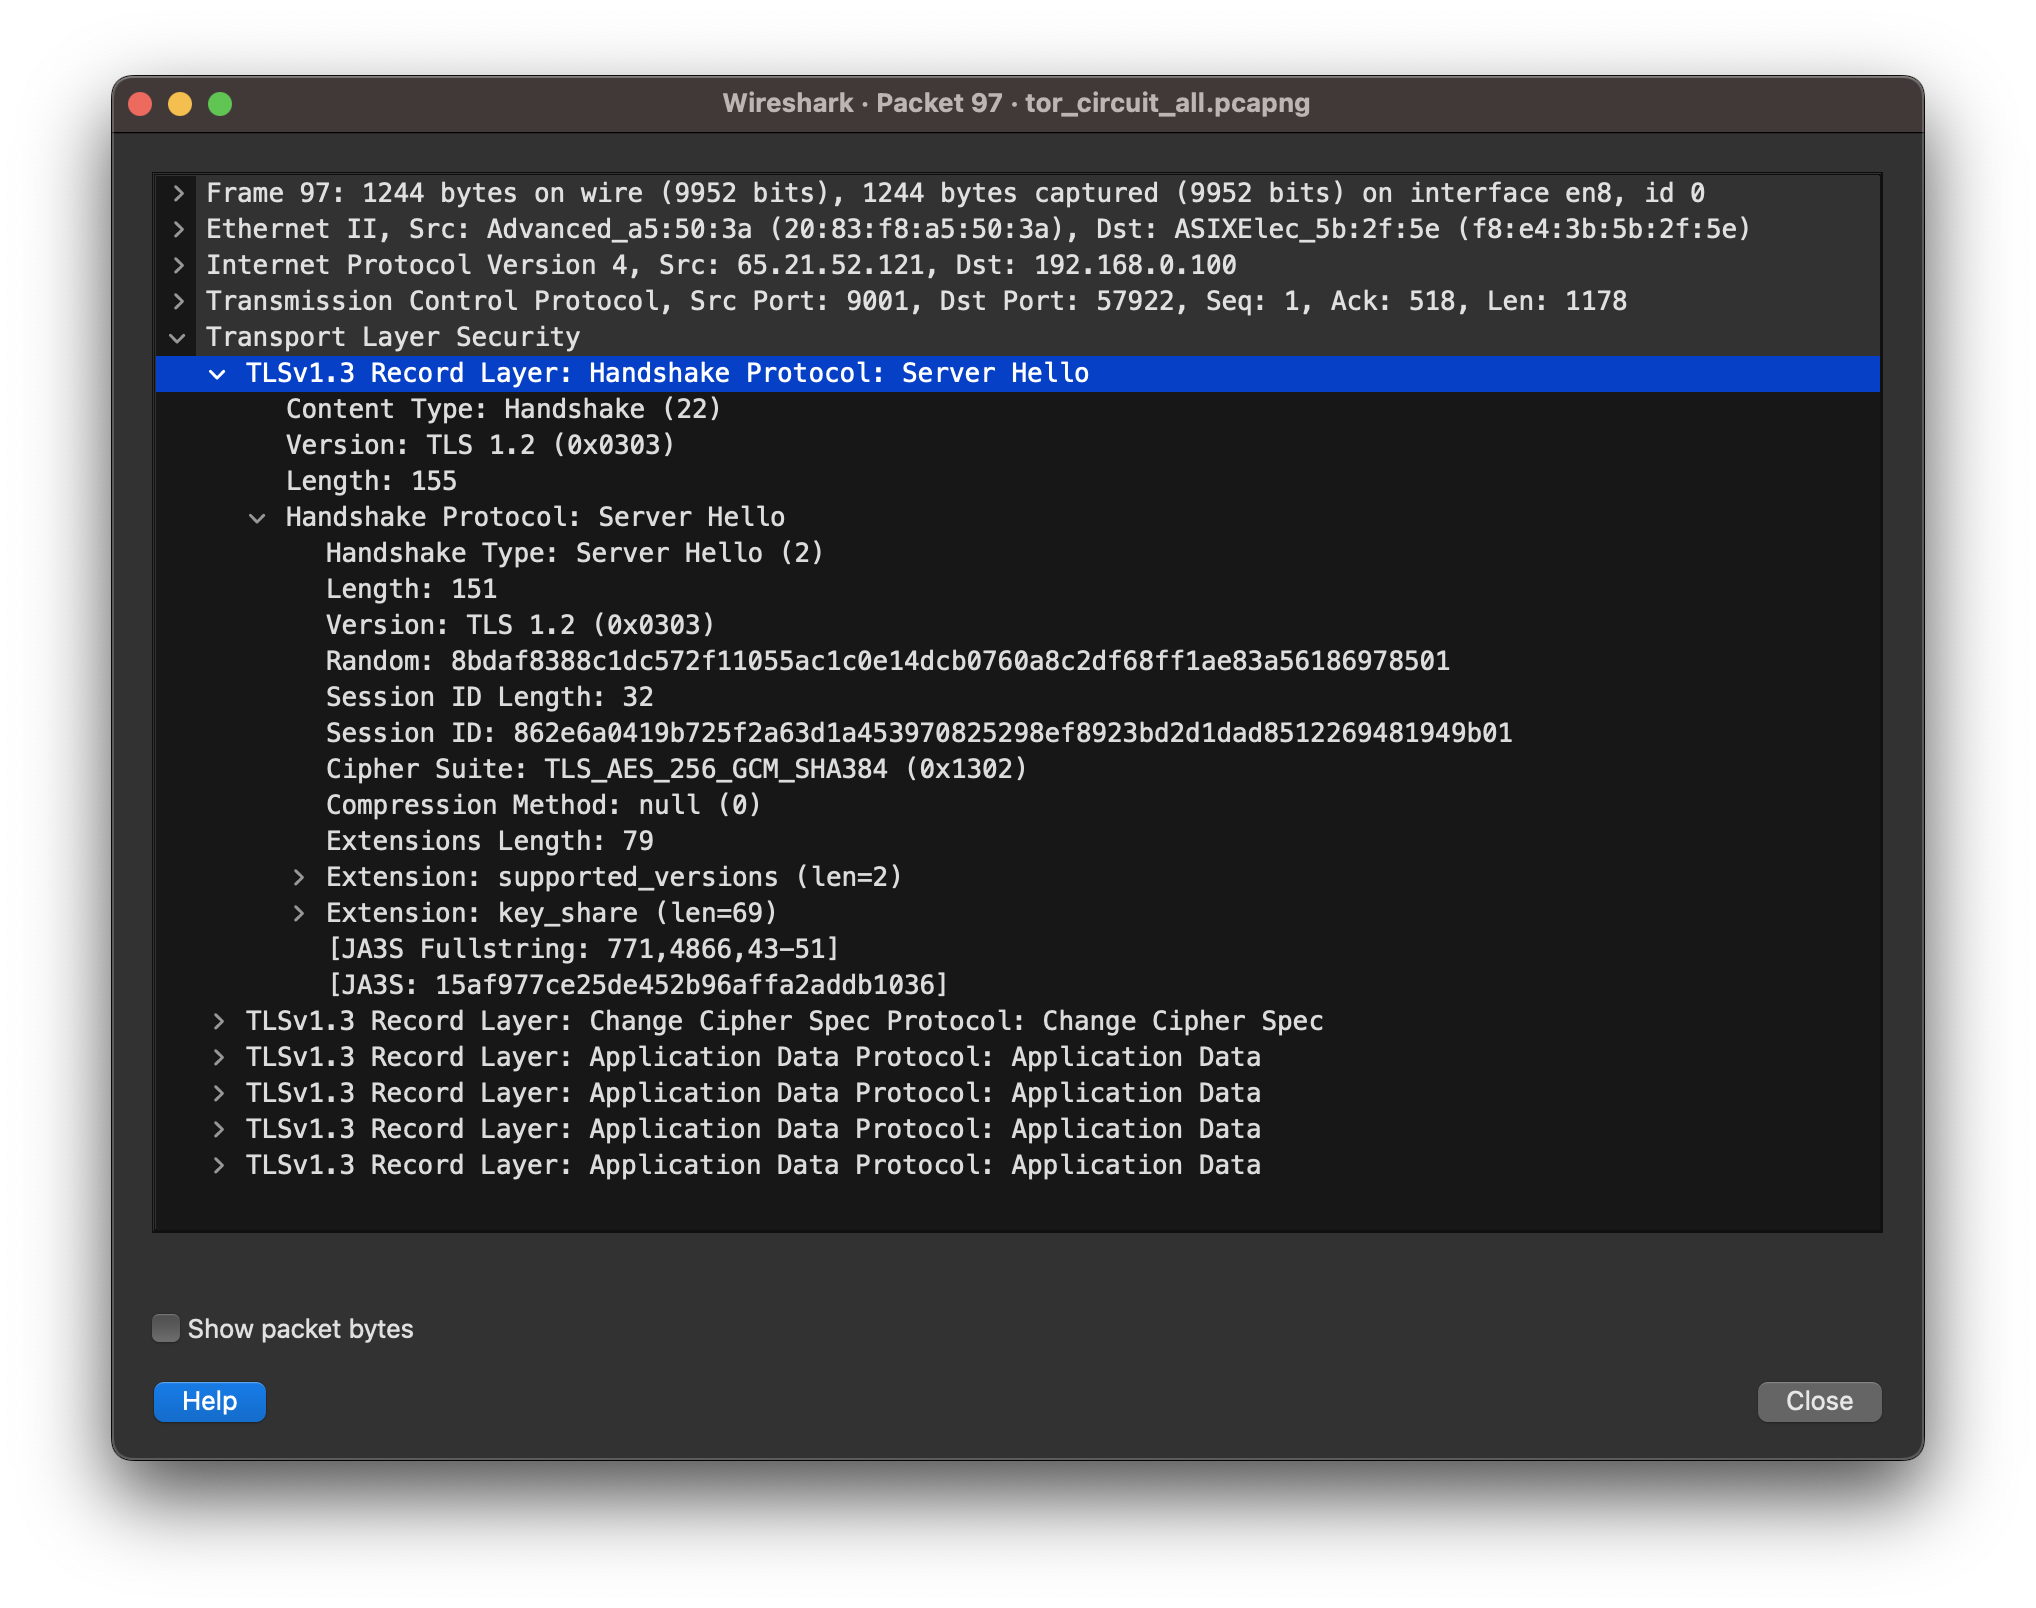
\includegraphics[width=\textwidth]{Wireshark/Server_Hello}
        \end{subfigure}
    \end{figure}
\end{frame}

\subsection{Chaum Mix}
\begin{frame}{Chaum Mix}
    La rete Onion è basata sullo studio di David Chaum che propose un sistema di comunicazione anonima basato sulla crittografia. Nella sua conclusione una rete di questo tipo doveva avere le seguenti caratteristiche:
    \begin{itemize}
        \item \textbf{Sealing}, una tecnica con cui il messaggio viene annesso ad una stringa casuale prima di essere criptato per aumentarne la sicurezza.
        \item \textbf{Indirizzo non tracciabile}, un indirizzo generato dal client criptando quello reale, rendendone possibile la decrittazione solo dal primo nodo. Viene usato come indirizzo di risposta dal destinatario.
    \end{itemize}
\end{frame}